\documentclass[12pt]{article}
    \usepackage[margin=1in]{geometry}
    \usepackage{mdframed}
    \usepackage{subcaption}
    \usepackage{amssymb}
    \usepackage{amsmath}
    \usepackage{mathtools}

    % Custom colors
    \usepackage{color}
    \definecolor{deepblue}{rgb}{0,0,0.5}
    \definecolor{deepred}{rgb}{0.6,0,0}
    \definecolor{deepgreen}{rgb}{0,0.5,0}
    % Default fixed font does not support bold face
    \DeclareFixedFont{\ttb}{T1}{txtt}{bx}{n}{12} % for bold
    \DeclareFixedFont{\ttm}{T1}{txtt}{m}{n}{12}  % for normal
    \usepackage{listings}
    \usepackage{url}

    \usepackage{hyperref}

    \usepackage{booktabs}
    
    \usepackage{tikz}
    \usetikzlibrary{shapes,arrows,automata,positioning,cd}
    \tikzset{
      cfgedge/.style   = {black, ->, >=stealth},
      forward/.style = { blue, ->, >=angle 45},
      backward/.style = { red, densely dashed, ->, >=latex' },
      backwardleft/.style = { red, densely dashed, <-, >=latex' },
    }
    \usepackage{xcolor}
    
    \newcommand{\cfgarrow}{\mathbin{\tikz[baseline]\draw[cfgedge,yshift=0.6ex] (0,0) -- (.9em,0);}}
    \newcommand{\forwardarrow}{\mathbin{\tikz[baseline]\draw[forward,yshift=0.6ex] (0,0) -- (1em,0);}}
    \newcommand{\backwardarrow}{\mathbin{\tikz[baseline]\draw[backward,yshift=0.6ex] (0,0) -- (.95em,0);}}
  \newcommand{\dom}{\underline{\gg}}
    
    
    \begin{document}

    \lstset{
    language=C,
    basicstyle=\ttfamily\small,
    keywordstyle=\ttb\color{deepblue}\small,
    emph={foo,bar,assert,baz},          % Custom highlighting
    emphstyle=\ttb\color{deepred}\small,    % Custom highlighting style
    stringstyle=\color{deepgreen}\small,
    frame=tb,                         % Any extra options here
    numbers=left,
    stepnumber=1,
    showstringspaces=false            % 
    }

    \begin{center}
        \bigskip
        {\LARGE ECS 240 Programming Languages} \medskip
                
        {\Large Homework 2} \bigskip
    
    \end{center}

    \section*{About This Assignment}
    
    \begin{itemize}
      \item This assignment tests you on your understanding of points-to analysis.
      \item To complete the assignment (i)~modify \texttt{hw2.tex}, (ii)~create
      the corresponding PDF document (using pdflatex, for example), and
      (iii)~submit the pdf electronically via Gradescope by the due date; see
      \href{https://www.gradescope.com/get_started#student-submission}{this page}
      and
      \href{http://gradescope-static-assets.s3-us-west-2.amazonaws.com/help/submitting_hw_guide.pdf}{this
      document}. Your assignment will not be graded and you will receive no
      points if you do not follow these instructions. 

      \item \textbf{When submitting the assignment on Gradescope, please mark
      which page corresponds to each question on the assignment.}  Your
      assignment will not be graded and you will receive no points if you do not
      mark the pages.      

      \item The  \LaTeX\ source has \texttt{TODO}~comments to clearly indicate
      where changes need to be made. 
      \item The \verb=\vspace= commands can be safely commented out.
      \item This assignment can be worked on in a group of at most three. Enter
      the names and email addresses of the team members in the space provided
      below.
    \end{itemize}

    \begin{mdframed}
      Team members:
      \begin{itemize}
        %TODO
        \item Divyansh Rajesh Jain, drajeshjain@ucdavis.edu % Enter name and email address of first team member.
        \item Soham Kolhatkar, sakolhatkar@ucdavis.edu % Comment out this line if working individually.
      \end{itemize}
    \end{mdframed}
    
    \newpage
    \begin{enumerate}
        \item (5 points) Consider the following C function:
        \begin{lstlisting}
          void bar(int *p, int *q) {
            if (*p != *q) return;
            (*q)++;
            (*p)++;
            (*q)++;
            // P1
          }
        \end{lstlisting}
        A program analyzer $A$ reports the following expression as an invariant
        at program point \lstinline$P1$: \lstinline$*p < *q$.

        Based solely on this report, state whether the following statement is
        \textbf{True} or \textbf{False}: 

        \emph{The program analyzer $A$ is sound.}

        If \textbf{True}, explain your reasoning. If \textbf{False}, provide an
        input for \lstinline$bar$ for which the expression evaluates to false.
         \begin{mdframed}
        %% TODO Comment out the correct answer.
        %\textbf{True} 
        \textbf{False}
        \begin{lstlisting}
          int a = 0;
          bar(&a, &a);
        \end{lstlisting}

        The above input to bar, where both p and q point to the same location, the statement $*p < *q$ will not be true, because after all the increments, *p would still equal *q.

        Therefore, since the invariant produced by the static analyzer doesn't hold for all inputs, the program analyzer $A$ is not sound.
        \end{mdframed}

        \item (5 points) Write down the set of statements $S$ such that performing precise flow-insensitive points-to
        analysis results in the following realizable pairs:\\
        $\{\langle a, r\rangle,\langle p, b\rangle,  \langle a, b\rangle, \langle p, r\rangle\}$.
        The size of $S$ should be \emph{at most 3}.
        \begin{mdframed}
          %% TODO At most three statements in S.
          $S = \{a = \&r, a = \&b, p = a\}$
          \end{mdframed}


        \item (5 points) Write down a program $P$ such that the output of a precise
        flow-sensitive points-to analysis at the end of the program $P$ is more
        precise compared to that of a precise flow-insensitive points-to
        analysis for the same program; that is, there are fewer points-to relations 
        inferred by flow-sensitive points-to analysis at the end of $P$ compared 
        to those inferred by precise flow-insensitive points-to analysis.
        
        Apart from the program $P$, your answer should also list the points-to 
        relations inferred by flow-sensitive and flow-insensitive analysis.

        \begin{mdframed}
          \vspace{4em}
          %% TODO
          %% Program P
          \textbf{Program P}

          \begin{lstlisting}
            void foo() {
              int a, b;
              void *c, p;

              //Statements
              c = &a;
              c = &b;
              p = c;
              //End of Program
            }
          \end{lstlisting}
          %% Points-to relations at end of P using flow-sensitive analysis
          \textbf{Points-to relations Precise Flow-Sensitive Analysis at End of Program}

          $\{\langle c, b\rangle,\langle p, b\rangle\}$
          %% Points-to relations using flow-insensitive analysis

          \textbf{Points-to relations Precise Flow-Insensitive Analysis}
          
          $\{\langle c, a\rangle, \langle c, b\rangle,\langle p, a\rangle\, \langle p, b\rangle\}$
        \end{mdframed}

      \item (5 points) A statement involving multiple dereferences can be broken
      into multiple statements each with a single deference involving temporary
      variables. Given a program $P$, let $OneStar(P)$ denote such a rewrite.
      For example, if $P \coloneqq$ \lstinline$y = &z; x = ***y$, then
      $OneStar(P) \coloneqq $ \lstinline$y = &z; t2 = *y; t1 = *t2; x = *t1;$.
      This rewrite does not reduce the precision of flow-sensitive points-to
      analysis. However, it could lead to imprecision for flow-insensitive
      points-to analysis; that is, performing precise flow-insensitive analysis
      on $P$ could produce fewer points-to relations compared to performing
      precise flow-insensitive analysis on $OneStar(P)$ even when we just
      consider the points-to relations among the variables of $P$.

      Give an example of a program $P$ such that precise flow-insensitive
      points-to analysis of $P$ is more precise compared to that for
      $OneStar(P)$ when considering \emph{only} the variables in $P$. Apart from
      $P$, your answer should also list $OneStar(P)$ and the points-to relations
      corresponding to $P$ and $OneStar(P)$.
      
      \begin{mdframed}
        \vspace{2em}
        %% TODO
        %% Program P
        %% Points-to relations for P using flow-insensitive analysis
        %% Program OneStar(P)
        %% Points-to relations for OneStar(P) using flow-insensitive analysis
      \end{mdframed}

      \item (5 points) Recall that a \emph{program with well-defined types}
      contains only variables that are scalars with well-defined types (e.g.
      \lstinline$int$, \lstinline$int*$, \lstinline$int**$, etc.). Furthermore,
      a variable can only point to variables of compatible type. For example, a
      variable of type \lstinline$int**$ can only point to a variable of type
      \lstinline$int*$, and a variable of type \lstinline$int*$ can only point
      to a variable of type \lstinline$int$.
      
      For a given program \textbf{P}, the following \emph{realizability graph}
      $G_R$ is constructed by computing precise flow-insensitive points-to
      analysis for \textbf{P}:
      \vspace{-2ex}
      \begin{center}
      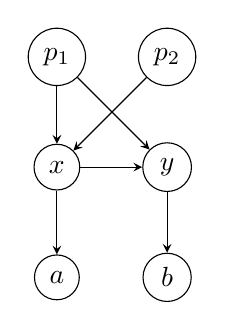
\begin{tikzpicture}[auto,
        node distance=1.4cm, 
        ] 
        \tikzstyle{every node} = [circle, draw]
        \node (p1) {$p_1$};
        \node [right of=p1] (p2) {$p_2$};
        \node [below of=p1] (x) {$x$};
        \node [below of=p2] (y) {$y$};
        \node [below of=x] (a) {$a$};
        \node [below of=y] (b) {$b$};
        
        \path (p1) edge[cfgedge] (x); 
        \path (p1) edge[cfgedge] (y); 
        \path (p2) edge [cfgedge] (x);
        \path (x) edge[cfgedge] (y); 
        \path (x) edge [cfgedge] (a);
        \path (y) edge [cfgedge] (b);    
        
        \end{tikzpicture}
      \end{center}
      \vspace{-1ex}
        Based on $G_R$, mark (using $\checkmark$) \textbf{EXACTLY ONE} statement
        from below that is true for program~\textbf{P}, and \textbf{justify your
        answer}:
        \vspace{-2ex}
        \renewcommand{\arraystretch}{1.5}
        \begin{center}
        \begin{tabular}{|l|l|}
          \hline
          The program \textbf{P} might be a program with well-defined types. & \hspace{3em} \\ \hline
          The program \textbf{P} is definitely NOT a program with well-defined types. & $\checkmark$ \\ \hline 
        \end{tabular}
      \end{center}
      \vspace{-2ex}
       \begin{mdframed}
        Justification for answer:

        In a program with well-defined types, a pointer with type n can only point to a variable with type n - 1. This means that in the realizability graph, we should only see edges from between nodes that are one level apart. But in the realizability graph above, we can see that there is an edge from x to y, where x and y are at the same level.

        Therefore, we know for a fact that this is not a program with well-defined types.
       \end{mdframed}
    

    \end{enumerate}
    
\end{document}